\documentclass[a4paper,oneside,12pt]{report}

\usepackage{tabularx}
\usepackage{booktabs}
\newcolumntype{Y}{>{\raggedright\arraybackslash}X}
\usepackage{fontspec}
\IfFontExistsTF{Times New Roman}{%
  \setmainfont{Times New Roman}%
}{%
  \setmainfont{texgyretermes-regular.otf}[
    BoldFont=texgyretermes-bold.otf,
    ItalicFont=texgyretermes-italic.otf,
    BoldItalicFont=texgyretermes-bolditalic.otf
  ]%
}
\usepackage{amsmath}
\usepackage{setspace}
\usepackage{graphicx}
\usepackage{titling}
\usepackage{geometry}
\usepackage{listings}
\usepackage{xcolor}
\usepackage{float}
\usepackage{indentfirst}
\usepackage{xurl}
\usepackage{hyperref}
\usepackage{fancyhdr}
\usepackage{tocloft}
\usepackage{bookmark}
\usepackage{microtype}

\onehalfspacing

\geometry{left=3cm, right=2.5cm, top=2cm, bottom=2.5cm}
\emergencystretch=3em
\hfuzz=1.5pt
\hbadness=10000
\hyphenpenalty=10000
\exhyphenpenalty=10000

\newcommand{\customfbox}[1]{%
  \setlength{\fboxsep}{0pt}%
  \setlength{\fboxrule}{0.5pt}%
  \fcolorbox{black}{white}{#1}%
}
\renewcommand{\figurename}{Gambar}
\renewcommand{\thefigure}{\arabic{figure}}
\renewcommand{\tablename}{Tabel}
\renewcommand{\thetable}{\arabic{table}}
\renewcommand{\theequation}{\arabic{equation}}
\hypersetup{
    colorlinks=true,
    linkcolor=black,
    filecolor=black,
    urlcolor=black,
    citecolor=black,
    pdftitle={Laporan Praktikum PPG Pertemuan 7},
    pdfpagemode=UseOutlines,
    breaklinks=true
}
\pagestyle{fancy}
\fancyhf{}
\fancyfoot[C]{\thepage}
\renewcommand{\headrulewidth}{0pt}
\fancypagestyle{plain}{
    \fancyhf{}
    \fancyfoot[C]{\thepage}
    \renewcommand{\headrulewidth}{0pt}
}
\renewcommand{\contentsname}{Daftar Isi}
\renewcommand{\bibname}{Daftar Pustaka}
\renewcommand{\thechapter}{}
\renewcommand{\chaptername}{}
\renewcommand{\thesection}{\arabic{chapter}.\arabic{section}}
\renewcommand{\thesubsection}{\thesection.\arabic{subsection}}
\setcounter{secnumdepth}{3}
\setcounter{tocdepth}{3}
\renewcommand{\cftchapdotsep}{\cftdotsep}
\renewcommand{\cftchapleader}{\cftdotfill{\cftchapdotsep}}
\setlength{\cftchapindent}{0em}
\setlength{\cftsecindent}{2em}
\setlength{\cftsubsecindent}{4em}
\setlength{\cftchapnumwidth}{0em}
\setlength{\cftsecnumwidth}{2.5em}
\setlength{\cftsubsecnumwidth}{3.2em}
\renewcommand{\cftchappresnum}{}
\renewcommand{\cftchapaftersnum}{}
\newcommand{\tocboldsection}[1]{%
  \protect\renewcommand{\protect\cftchapfont}{\protect\bfseries}%
  #1%
  \protect\renewcommand{\protect\cftchapfont}{}%
}
\pdfstringdefDisableCommands{\def\tocboldsection#1{#1}}

\begin{document}

% Halaman Judul
\newgeometry{left=3cm, right=2.5cm, top=2.5cm, bottom=3cm}
\begin{titlingpage}
	\begin{spacing}{1}
		\begin{center}
			\vspace*{0.2cm}
			{\large \textbf{\MakeUppercase{Laporan Praktikum}}} \\[0.4cm]
			{\large \textbf{\MakeUppercase{PRAKTIKUM PENGEMBANGAN GAME}}} \\[0.4cm]
			{\large \textbf{\MakeUppercase{Pertemuan 7}}} \\[0.4cm]
			{\large \textbf{\MakeUppercase{ASSET FAB DAN WIDGET BLUEPRINT (UI)}}} \\[1.5cm]

			
\includegraphics[height=7cm]{images/UGM.png} \\[0.7cm]

			{\normalsize \textbf{Disusun oleh:}} \\[0.4cm]
			\begin{tabular}{@{}l l @{}}
				\textbf{Nama}           & : Hafidz Rizqullah Prasetya                   \\
				\textbf{NIM}            & : 24/535493/SV/24243                          \\
				\textbf{NIU}            & : 535493                                      \\
				\textbf{Kelas}          & : PL5A1                                       \\
				\textbf{Dosen Pengampu} & : Yusron Fuadi, S.Sn., M.Sn.                  \\
				\textbf{Asisten}        & : Ezra Bariq Rizqullah / Ikhwan Hanif Firdaus \\
			\end{tabular} \\[1.2cm]

			{\normalsize \textbf{PROGRAM STUDI D-IV}} \\[0.2cm]
			{\normalsize \textbf{TEKNOLOGI REKAYASA PERANGKAT LUNAK}} \\[0.2cm]
			{\normalsize \textbf{DEPARTEMEN TEKNIK ELEKTRO DAN INFORMATIKA}} \\[0.2cm]
			{\normalsize \textbf{SEKOLAH VOKASI}} \\[0.2cm]
			{\normalsize \textbf{UNIVERSITAS GADJAH MADA}} \\[0.2cm]
			{\normalsize \textbf{YOGYAKARTA}} \\[0.2cm]
			{\normalsize \textbf{2026}} \\[1.2cm]
		\end{center}
	\end{spacing}
\end{titlingpage}
\restoregeometry

\thispagestyle{empty}
\clearpage
\stepcounter{page}
\thispagestyle{empty}

%  --- Daftar Isi ---
\addcontentsline{toc}{chapter}{Daftar Isi}
\tableofcontents
\clearpage

\pagenumbering{arabic}
\setcounter{page}{3}

\chapter[Tujuan Praktikum]{Tujuan Praktikum}
\begin{enumerate}\setlength{\itemsep}{0.3em}\setlength{\parskip}{0pt}
	\item Mahasiswa mampu melakukan eksplorasi, pengunduhan, serta integrasi aset lingkungan tiga dimensi dari marketplace terpadu Fab ke dalam proyek Unreal Engine 5.8 \cite{modul7,fab-market}.
	\item Mahasiswa mampu mengonfigurasi dan mengaplikasikan material bentang alam multi-layer (\textit{Landscape Material}) menggunakan kontainer data \textit{Layer Info} untuk kebutuhan pengecatan tekstur permukaan lingkungan \cite{modul7,epic-landscape-materials}.
	\item Mahasiswa mampu menerapkan aset vegetasi lingkungan (\textit{foliage}) secara presisi melalui metode penempatan manual maupun secara prosedural memanfaatkan \textit{Foliage Mode} \cite{modul7,epic-foliage-mode}.
	\item Mahasiswa mampu merancang antarmuka visual pemain (\textit{User Interface}) berbasis UMG (\textit{Unreal Motion Graphics}), mencakup penataan hierarki kanvas, batang status kesehatan (\textit{HealthBar}), serta animasi respons visual dinamis \cite{modul7,epic-umg,epic-widget-animation}.
	\item Mahasiswa mampu mengintegrasikan sistem antarmuka ke dalam siklus hidup permainan secara modular melalui implementasi \textit{Blueprint Interface} dan \textit{Game Instance}, menghubungkan penurunan nilai darah pemain saat menerima luka langsung ke indikator layar \cite{modul7,epic-blueprint-interface,epic-game-instance}.
\end{enumerate}
\clearpage

\chapter{Dasar Teori}

\section{Ekosistem Fab dan Distribusi Aset Digital Terpadu}
Industri pengembangan game modern sangat bergantung pada ketersediaan pustaka aset digital berkualitas tinggi guna mempercepat fase prototipe dan produksi \cite{fab-market}. Epic Games meluncurkan platform Fab sebagai pasar digital terpadu yang menggabungkan berbagai ekosistem aset terdahulu, seperti Unreal Engine Marketplace, Sketchfab, ArtStation Marketplace, dan Quixel \cite{epic-fab-overview}. Penyatuan ini menghadirkan repositori aset tiga dimensi agnostik yang dapat dimanfaatkan lintas perangkat lunak kreasi konten, mulai dari Unreal Engine, Unity, Blender, hingga Maya \cite{fab-market}.

Dalam konteks kompatibilitas versi, paket aset lingkungan seperti \textit{Landscape Pro 2.0} umumnya dirilis untuk versi engine tertentu (misalnya UE 5.5). Unreal Engine menyediakan mekanisme impor adaptif yang memungkinkan pengembang memuat aset dari versi terdahulu ke dalam engine mutakhir (UE 5.8) \cite{modul7}. Melalui jendela konfigurasi Library, aset dikonversi secara transparan ke format uasset lokal, memastikan shader, material instanced, dan hierarki static mesh tetap utuh tanpa merusak integritas berkas proyek \cite{modul7}.

\section{Arsitektur Material Landscape Multi-Layer dan Layer Info}
Bentang alam pada Unreal Engine membutuhkan penanganan material khusus yang mampu membaurkan berbagai jenis tekstur permukaan (seperti tanah, rumput, lumpur, dan bebatuan) pada koordinat medan yang sama \cite{epic-landscape-materials}. Sistem ini diimplementasikan melalui material berlapis (\textit{Landscape Material}) yang memanfaatkan ekspresi \texttt{Landscape}\allowbreak\texttt{LayerBlend} \cite{epic-landscape-materials}.

\begin{equation}
	\mathbf{C}_{\text{final}}(u,v) = \sum_{i=1}^{N} w_i(u,v) \cdot \mathbf{C}_i(u,v)
\end{equation}

Persamaan di atas merepresentasikan kalkulasi warna permukaan akhir $\mathbf{C}_{\text{final}}$ pada titik koordinat UV $(u,v)$, di mana $\mathbf{C}_i$ merupakan nilai warna difus dari layer material ke-$i$, dan $w_i$ adalah faktor bobot (\textit{weight}) sapuan kuas yang ternormalisasi ($\sum w_i = 1$). Agar sistem rendering mampu menyimpan dan mengevaluasi bobot sapuan cat pada setiap titik verteks secara persisten, Unreal Engine memerlukan kontainer data yang disebut \textit{Layer Info} \cite{modul7}. Objek aset ini menyimpan parameter fisik permukaan (seperti respon jejak kaki dan gesekan fisika) serta memori alokasi bobot blending, sehingga lapisan cat yang berbeda dapat dipadukan secara mulus di atas satu mesh landscape yang sama \cite{epic-landscape-materials}.

\section{Distribusi Vegetasi Lingkungan Melalui Foliage System}
Vegetasi lingkungan (\textit{foliage}) mencakup pepohonan, semak-semak, dan rerumputan yang memberikan kepadatan visual pada dunia game terbuka \cite{epic-foliage-mode}. Unreal Engine menyediakan dua metodologi penempatan foliage:
\begin{enumerate}\setlength{\itemsep}{0.15em}\setlength{\parskip}{0pt}
	\item \textbf{Penempatan Manual (\textit{Manual Placement})}: Penempatan static mesh secara langsung melalui proses seret dan lepas (\textit{drag-and-drop}) dari Content Drawer ke level. Metode ini memberikan kontrol tata letak presisi tinggi, umumnya diterapkan pada pohon-pohon signifikan (\textit{hero assets}) atau penanda navigasi visual \cite{modul7}.
	\item \textbf{Foliage Mode Painting}: Pendekatan instansiasi prosedural di mana sekumpulan \textit{Static Mesh Foliage} didaftarkan ke panel Foliage. Pengembang dapat mengecat vegetasi secara masif dengan parameter kerapatan (\textit{density}), skala acak (\textit{scaling}), orientasi rotasi acak, dan penyelarasan terhadap kemiringan normal permukaan tanah \cite{epic-foliage-mode}. Teknik ini mengelompokkan ribuan model ke dalam satu \textit{Hierarchical Instanced Static Mesh} (HISM) guna meminimalkan beban panggilan penggambaran grafis (\textit{draw calls}) \cite{epic-foliage-mode}.
\end{enumerate}

\section{Arsitektur User Interface Menggunakan UMG dan Animasi Widget}
Sistem antarmuka pengguna pada Unreal Engine dibangun menggunakan kerangka kerja \textit{Unreal Motion Graphics} (UMG) yang berbasis slate \cite{epic-umg}. Setiap antarmuka dienkapsulasi ke dalam \textit{Widget Blueprint}, yang memiliki dua mode kerja utama: mode \textit{Designer} untuk tata letak visual berbasis kanvas dan mode \textit{Graph} untuk pemrograman logika interaksi pemain \cite{epic-umg}.

Komponen \texttt{Canvas Panel} bertindak sebagai kontainer induk berorientasi koordinat absolut yang mendukung sistem penjangkaran (\textit{anchors}). Penjangkaran memastikan elemen UI (seperti indikator status di pojok kiri atas) tetap berada pada posisi proporsional terhadap berbagai rasio aspek monitor pemain \cite{epic-umg}. Di dalam kanvas tersebut, komponen visual seperti \texttt{Progress Bar} digunakan untuk menampilkan rasio metrik numerik kontinu (darah, stamina, energi). Nilai isian bar diatur melalui properti persentase:

\begin{equation}
	\text{Percent} = \text{clamp}\left(\frac{\text{CurrentHealth}}{\text{MaxHealth}}, 0.0, 1.0\right)
\end{equation}

Guna memperkaya umpan balik sensorik pemain (\textit{visual feedback}), UMG menyediakan panel editor linimasa \textit{Widget Animation} \cite{epic-widget-animation}. Pengembang dapat memanipulasi sub-jalur \textit{Transform (Translation X, Y)} untuk menghasilkan efek getaran cepat (\textit{shake/jiggle}) saat nilai darah mengalami perubahan, memperjelas persepsi bahaya saat karakter menerima kerusakan \cite{modul7}.

\section{Pemisahan Ketergantungan via Blueprint Interface dan Game Instance}
Dalam perancangan perangkat lunak game berorientasi objek, ketergantungan langsung antar-kelas (\textit{hard-casting}) merupakan pola anti-desain yang meningkatkan beban komputasi dan memicu kesalahan sirkular \cite{epic-blueprint-interface}. Unreal Engine mengatasi kendala ini melalui pemanfaatan \textit{Blueprint Interface} (BPI). BPI mendefinisikan kontrak fungsi tanpa implementasi konkret, memungkinkan komunikasi antar-aktor tanpa memerlukan referensi kelas spesifik \cite{epic-blueprint-interface}.

\begin{table}[H]
	\centering
	\renewcommand{\arraystretch}{1.25}
	\caption{Perbandingan komunikasi antar-Blueprint menggunakan Hard Casting versus Blueprint Interface \cite{epic-blueprint-interface,modul7}.}
	\label{tab:komparasi-casting-interface}
	\begin{tabularx}{\linewidth}{|l|Y|Y|}
		\hline
		\textbf{Parameter Evaluasi} & \textbf{Hard Casting (\texttt{Cast To})} & \textbf{Blueprint Interface (\texttt{BPI})} \\
		\hline
		Tingkat Ketergantungan & Sangat ketat (\textit{tightly coupled}); memuat referensi kelas ke memori. & Terisolasi penuh (\textit{loosely coupled}); referensi kelas tidak dimuat. \\
		\hline
		Penanganan Kegagalan & Memicu percabangan \textit{Cast Failed} jika target objek berbeda kelas. & Diabaikan secara aman tanpa pesan galat jika objek tidak mengimplementasikan interface. \\
		\hline
		Efisiensi Kompilasi & Perubahan pada kelas target memaksa rekompilasi seluruh pemanggil. & Perubahan internal kelas tidak memengaruhi penyeru pesan interface. \\
		\hline
		Aksesibilitas Objek & Terbatas pada hierarki pewarisan kelas yang sama atau subkelasnya. & Bersifat universal; dapat dipanggil ke sembarang aktor atau widget. \\
		\hline
	\end{tabularx}
\end{table}

Untuk mengelola referensi widget antarmuka secara global sepanjang sesi aplikasi, sistem memanfaatkan \textit{Game Instance} \cite{epic-game-instance}. Berbeda dengan aktor level atau Player Controller yang dapat dihancurkan saat perpindahan level, objek Game Instance tetap persisten di memori selama proses permainan berjalan. Menyimpan referensi widget di Game Instance via antarmuka memastikan sistem luar (seperti komponen karakter yang menerima damage) dapat memperbarui tampilan HUD secara instan tanpa perlu melacak hierarki viewport secara manual \cite{modul7,epic-game-instance}.

\clearpage

\chapter[\tocboldsection{Hasil dan Pembahasan}]{Hasil dan Pembahasan}

Praktikum Pertemuan 7 dilaksanakan menggunakan Unreal Engine 5.8 pada basis proyek \texttt{HAFIDZ\_535493\_PPG}. Praktikum ini melanjutkan pengembangan prototipe permainan dari pertemuan-pertemuan sebelumnya, dengan fokus mengintegrasikan aset bentang alam Fab, memperkaya lingkungan dengan vegetasi foliage, serta membangun sistem antarmuka status kesehatan pemain (HUD) berbasis UMG yang terhubung ke logika gameplay \cite{modul7}.

\section{Dokumentasi Praktikum}

\subsection{Eksplorasi FAB Marketplace dan Integrasi Aset Landscape Pro 2.0}

\begin{enumerate}\setlength{\itemsep}{0.5em}
	\item \textbf{Eksplorasi Aset pada Platform Fab.} Melalui aplikasi Epic Games Launcher, tab \textbf{Fab} dibuka untuk mengakses repositori aset digital terpadu. Pada bilah pencarian, kata kunci \textbf{Landscape Pro 2.0} dimasukkan untuk menemukan paket bentang alam multi-layer yang menyediakan pustaka tekstur tanah serta mesh vegetasi fotorealistik. Tampilan pencarian aset Fab diperlihatkan pada Gambar \ref{fig:ss-fab-browsing-landscapepro}.

	      \begin{figure}[H]
		      \centering
		      \customfbox{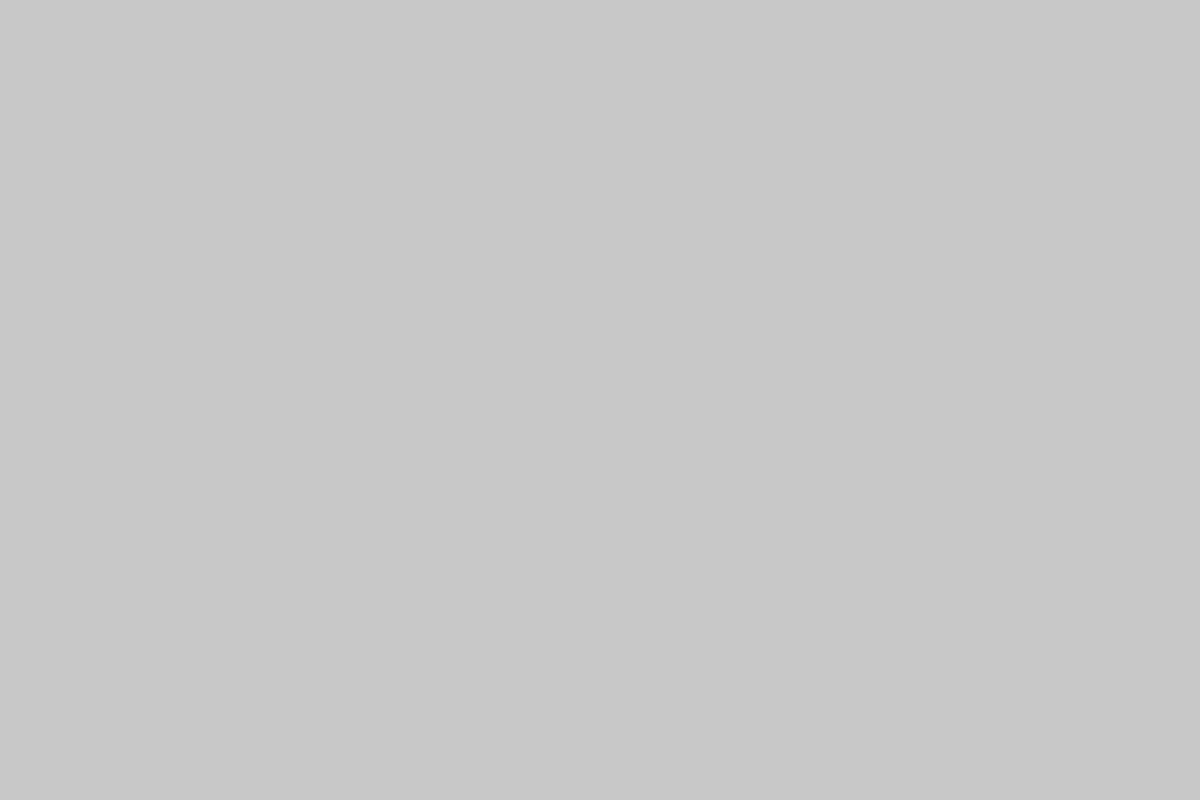
\includegraphics[width=0.63\textwidth,keepaspectratio]{images/ss-01-fab-browsing-landscapepro.png}}
		      \caption{Pencarian paket aset Landscape Pro 2.0 pada antarmuka marketplace digital Fab.}
		      \label{fig:ss-fab-browsing-landscapepro}
	      \end{figure}

	\item \textbf{Penambahan Aset ke Proyek Unreal Engine 5.8.} Paket aset \textit{Landscape Pro 2.0} secara resmi dirancang untuk Unreal Engine 5.5. Agar dapat digunakan pada lingkungan praktikum UE 5.8, jendela dialog \textbf{Add To Project} dibuka dari Fab Library. Opsi \textbf{Show all projects} diaktifkan, proyek praktikum \texttt{HAFIDZ\_535493\_PPG} dipilih, dan dropdown versi disetel secara eksplisit ke versi \textbf{5.5}. Proses penyesuaian versi ini ditunjukkan pada Gambar \ref{fig:ss-fab-add-to-project-version-55}.

	      \begin{figure}[H]
		      \centering
		      \customfbox{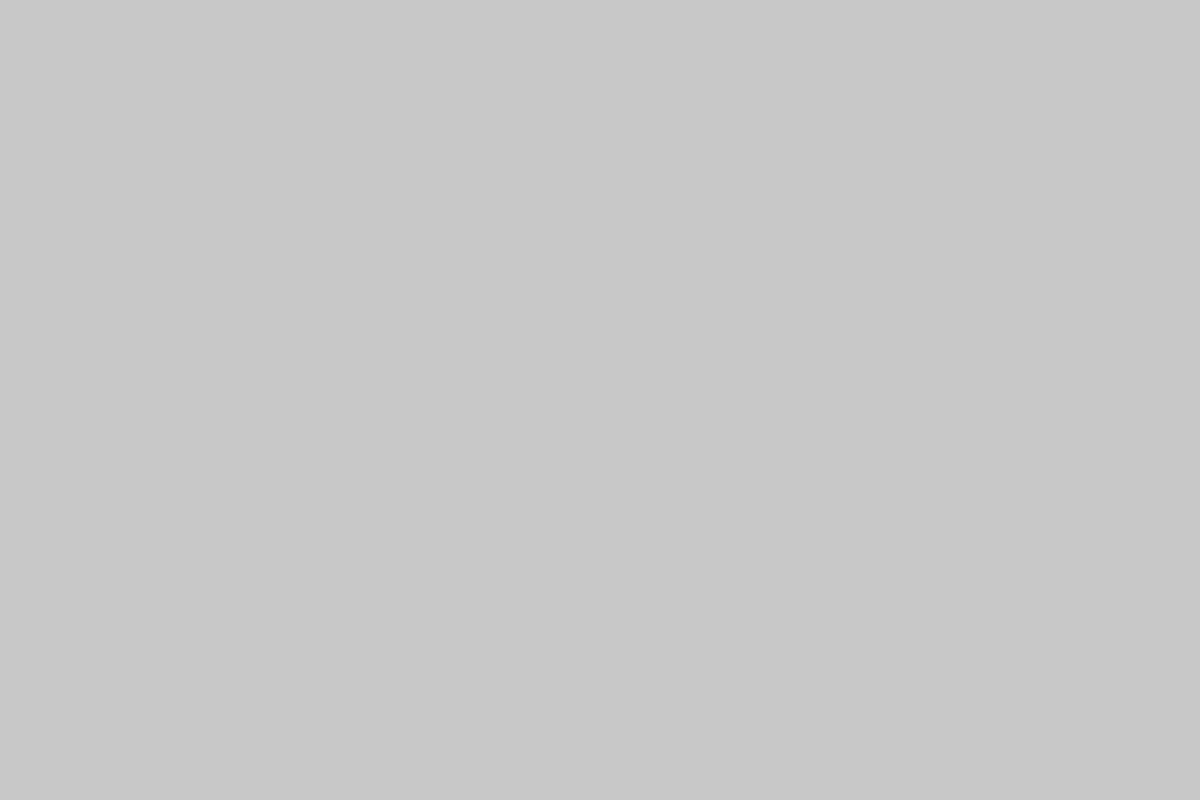
\includegraphics[width=0.63\textwidth,keepaspectratio]{images/ss-02-fab-add-to-project-version-55.png}}
		      \caption{Konfigurasi pengunduhan aset versi 5.5 ke dalam proyek target Unreal Engine 5.8.}
		      \label{fig:ss-fab-add-to-project-version-55}
	      \end{figure}

	\item \textbf{Inspeksi Berkas Foliage pada Content Drawer.} Setelah proses pengunduhan selesai dan indikator ukuran tembolok (\textit{Cache Size}) muncul, proyek dibuka kembali. Melalui Content Drawer, direktori penempatan aset diperiksa pada jalur \texttt{Content/STF/Pack03-LandscapePro/Environment/Foliage}. Filter jenis aset \textbf{Static Mesh} diaktifkan untuk menampilkan variasi model tiga dimensi pepohonan, ranting, dan semak belukar sebagaimana tampak pada Gambar \ref{fig:ss-content-drawer-foliage-assets}.

	      \begin{figure}[H]
		      \centering
		      \customfbox{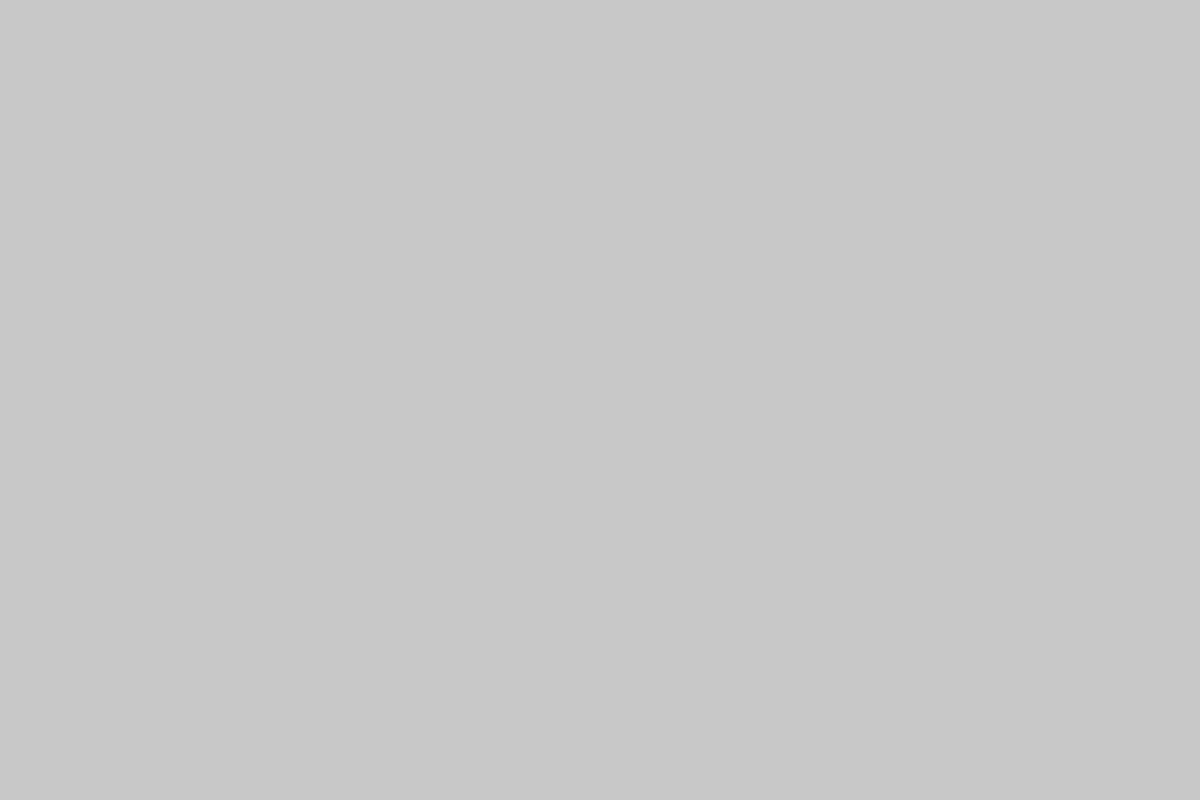
\includegraphics[width=0.63\textwidth,keepaspectratio]{images/ss-03-content-drawer-foliage-assets.png}}
		      \caption{Pemeriksaan model tiga dimensi vegetasi lingkungan pada direktori paket aset Landscape Pro.}
		      \label{fig:ss-content-drawer-foliage-assets}
	      \end{figure}
\end{enumerate}

\subsection{Implementasi Material Landscape dan Pengecatan Lapisan Permukaan}

\begin{enumerate}\setlength{\itemsep}{0.5em}\setcounter{enumi}{3}
	\item \textbf{Penerapan Material Multi-Layer pada Bentang Alam.} Berkas level praktikum \textbf{LV\_Praktikum} dibuka. Objek \texttt{Landscape} yang telah dibentuk konturnya pada pertemuan sebelumnya dipilih. Melalui panel \textbf{Details}, parameter \textbf{Landscape Material} diperbarui dengan menetapkan instans material bawaan paket, yaitu \textbf{MI\_landscape\_pro\_v2\_inst}. Tampilan panel Details dan pembaruan slot material ini diperlihatkan pada Gambar \ref{fig:ss-landscape-material-assigned}.

	      \begin{figure}[H]
		      \centering
		      \customfbox{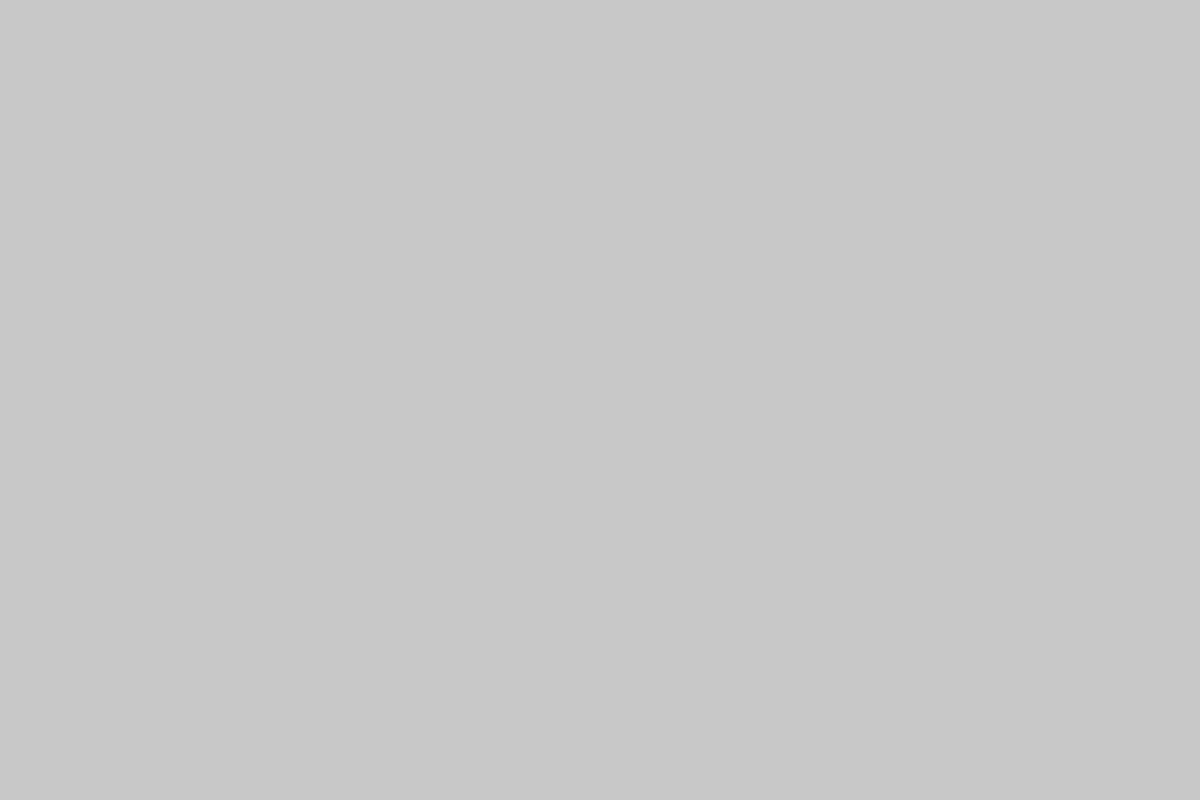
\includegraphics[width=0.63\textwidth,keepaspectratio]{images/ss-04-landscape-material-assigned.png}}
		      \caption{Penetapan material instanced MI\_landscape\_pro\_v2\_inst pada properti aktor Landscape.}
		      \label{fig:ss-landscape-material-assigned}
	      \end{figure}

	\item \textbf{Konfigurasi Layer Info pada Landscape Paint Mode.} Mode interaksi dialihkan ke \textbf{Landscape Mode} (\texttt{Shift + 2}) pada tab \textbf{Paint}. Tombol pengekstrakan otomatis diklik untuk memunculkan daftar lapisan material yang terdefinisi di dalam shader. Pada setiap layer yang berstatus \textit{None}, kontainer data \textbf{Layer Info} ditetapkan dari daftar opsi teratas guna mengaktifkan alur pencatatan bobot blending tekstur. Konfigurasi panel Paint ini ditampilkan pada Gambar \ref{fig:ss-landscape-paint-layer-info}.

	      \begin{figure}[H]
		      \centering
		      \customfbox{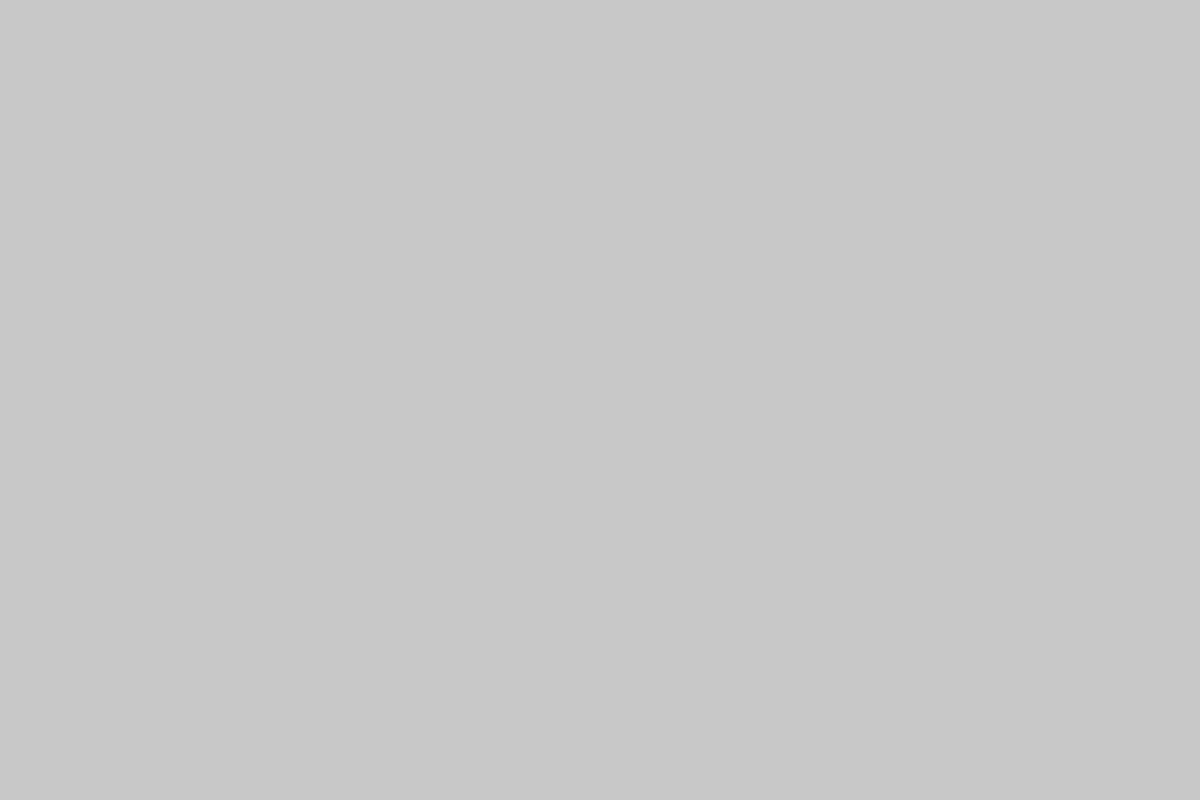
\includegraphics[width=0.63\textwidth,keepaspectratio]{images/ss-05-landscape-paint-layer-info.png}}
		      \caption{Penetapan kontainer data Layer Info untuk setiap lapisan material pada panel Landscape Paint.}
		      \label{fig:ss-landscape-paint-layer-info}
	      \end{figure}

	\item \textbf{Pengecatan Variasi Tekstur Bentang Alam.} Pengecatan kontur tanah dilakukan langsung pada viewport menggunakan kuas landscape. Variasi tekstur rumput (\textit{Grass}), tanah gersang (\textit{Ground}), dan genangan air (\textit{Puddle}) disapukan secara selektif untuk menciptakan kontras visual bentang alam yang alami. Gambar \ref{fig:ss-landscape-painting-variation} memperlihatkan hasil transisi gradasi tekstur permukaan yang terbentuk berkat evaluasi data bobot Layer Info.

	      \begin{figure}[H]
		      \centering
		      \customfbox{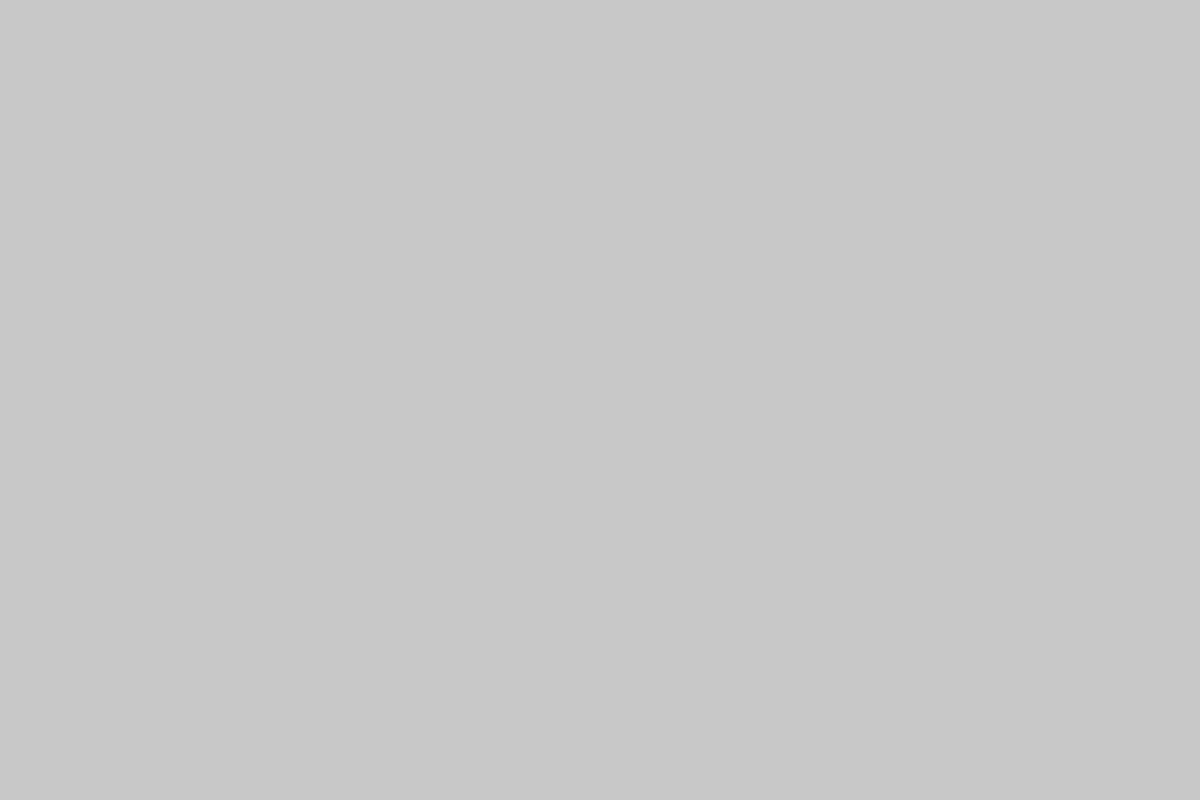
\includegraphics[width=0.63\textwidth,keepaspectratio]{images/ss-06-landscape-painting-variation.png}}
		      \caption{Tampilan permukaan bentang alam setelah proses pengecatan multi-layer tekstur tanah dan genangan.}
		      \label{fig:ss-landscape-painting-variation}
	      \end{figure}
\end{enumerate}

\subsection{Penerapan Vegetasi Foliage Manual dan Foliage Mode}

\begin{enumerate}\setlength{\itemsep}{0.5em}\setcounter{enumi}{6}
	\item \textbf{Penempatan Vegetasi Secara Manual.} Untuk menata pepohonan tertentu pada titik strategis di sekitar area awal pemain (\textit{Player Start}), model static mesh pohon dipilih dari Content Drawer lalu ditarik langsung ke atas permukaan tanah (\textit{drag-and-drop}). Metode penempatan manual ini memastikan orientasi dan skala pohon heroik tertata rapi tanpa tumpang tindih acak, seperti tampak pada Gambar \ref{fig:ss-foliage-manual-placement}.

	      \begin{figure}[H]
		      \centering
		      \customfbox{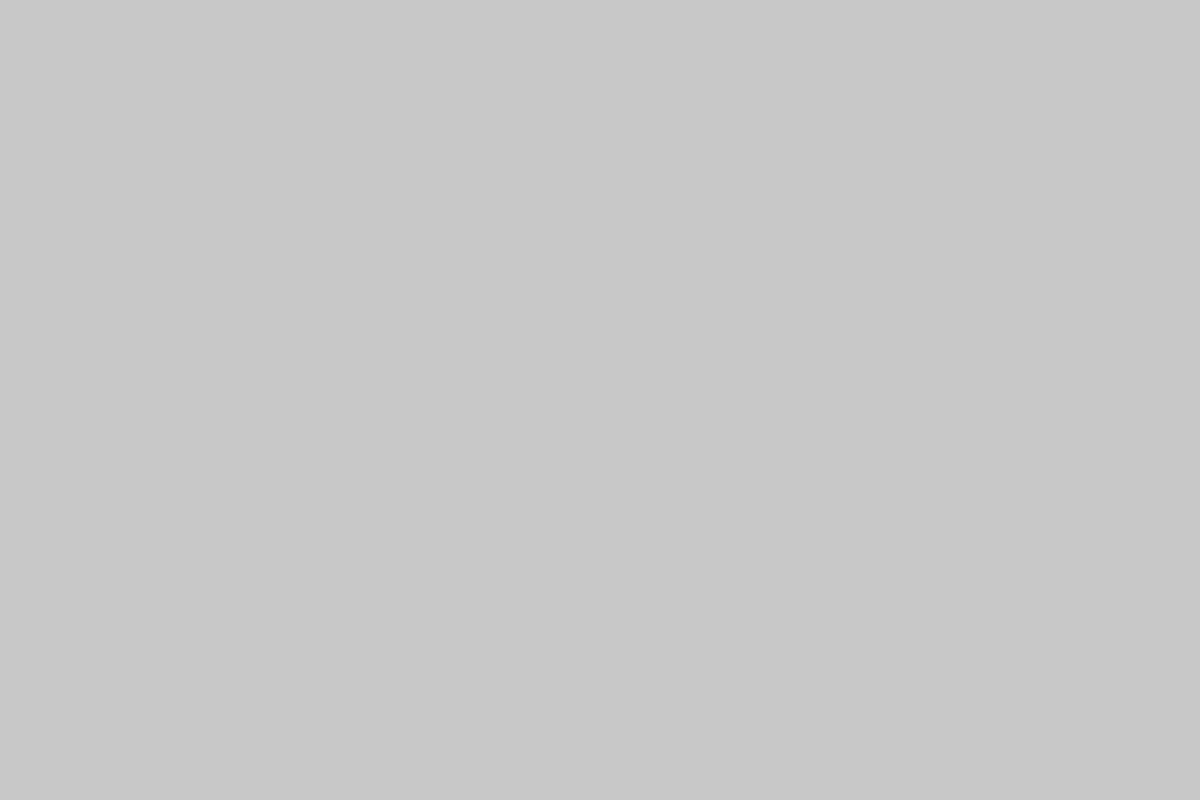
\includegraphics[width=0.63\textwidth,keepaspectratio]{images/ss-07-foliage-manual-placement.png}}
		      \caption{Penempatan model pepohonan secara manual pada koordinat bentang alam melalui Content Drawer.}
		      \label{fig:ss-foliage-manual-placement}
	      \end{figure}

	\item \textbf{Pengecatan Vegetasi Massal Menggunakan Foliage Mode.} Mode kerja dipindahkan ke \textbf{Foliage Mode} (\texttt{Shift + 3}). Seluruh aset bertipe \textit{Static Mesh Foliage} pada direktori paket ditarik ke dalam kotak penampung \textbf{Drop Foliage Here}. Jenis pohon yang diinginkan dicentang, dan sapuan kuas foliage diaplikasikan di atas bentang alam untuk menghasilkan sebaran hutan yang lebat dan efisien. Gambar \ref{fig:ss-foliage-mode-painting} memperlihatkan sebaran pohon hasil instansiasi prosedural tersebut.

	      \begin{figure}[H]
		      \centering
		      \customfbox{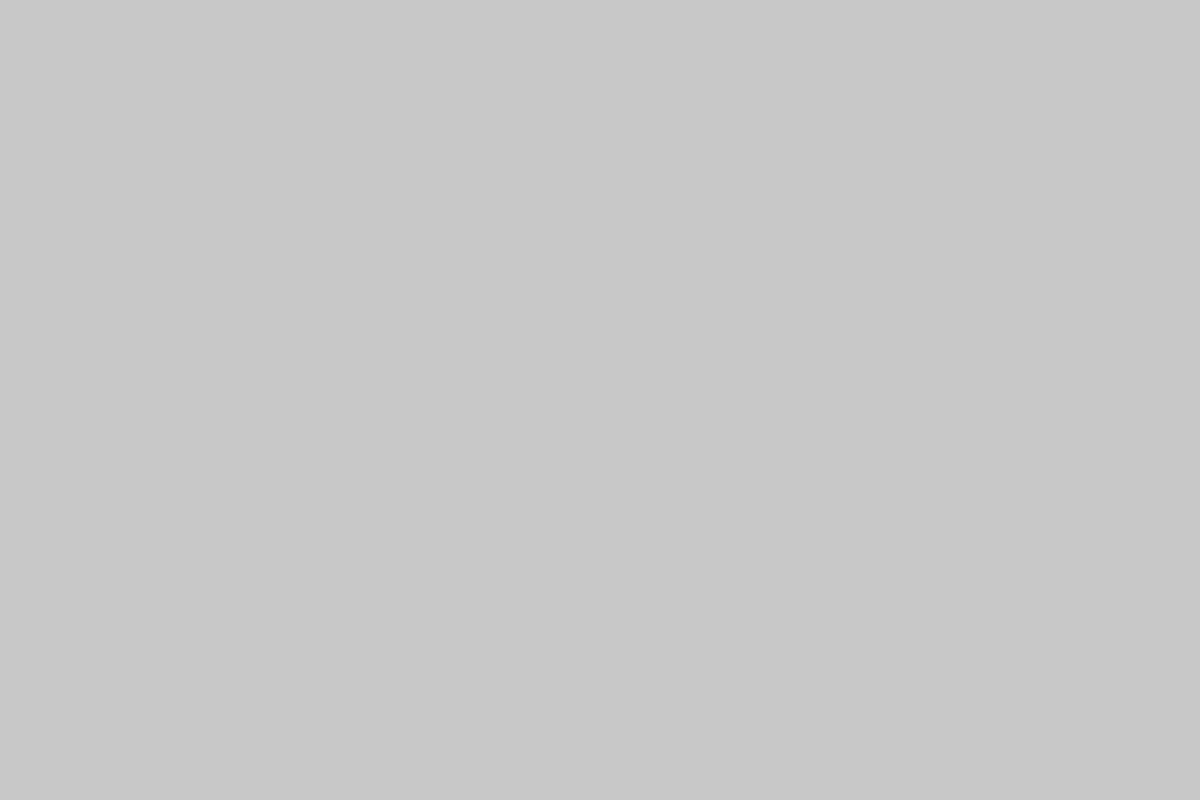
\includegraphics[width=0.63\textwidth,keepaspectratio]{images/ss-08-foliage-mode-painting.png}}
		      \caption{Pengecatan vegetasi massal menggunakan Foliage Mode pada area terbuka bentang alam.}
		      \label{fig:ss-foliage-mode-painting}
	      \end{figure}
\end{enumerate}

\subsection{Perancangan Widget Blueprint dan Animasi UI}

\begin{enumerate}\setlength{\itemsep}{0.5em}\setcounter{enumi}{8}
	\item \textbf{Pembuatan Berkas Widget Blueprint.} Struktur direktori proyek dirapikan dengan membuat folder baru bernama \textbf{Widget} di bawah direktori \texttt{Content}. Melalui menu \textbf{Add > User Interface > Widget Blueprint}, dua berkas User Widget dibuat, yaitu \textbf{WBP\_HUD} sebagai kanvas antarmuka utama dan \textbf{WBP\_Health} sebagai modul penampil bar darah pemain. Susunan berkas ini diperlihatkan pada Gambar \ref{fig:ss-create-wbp-hud-and-health}.

	      \begin{figure}[H]
		      \centering
		      \customfbox{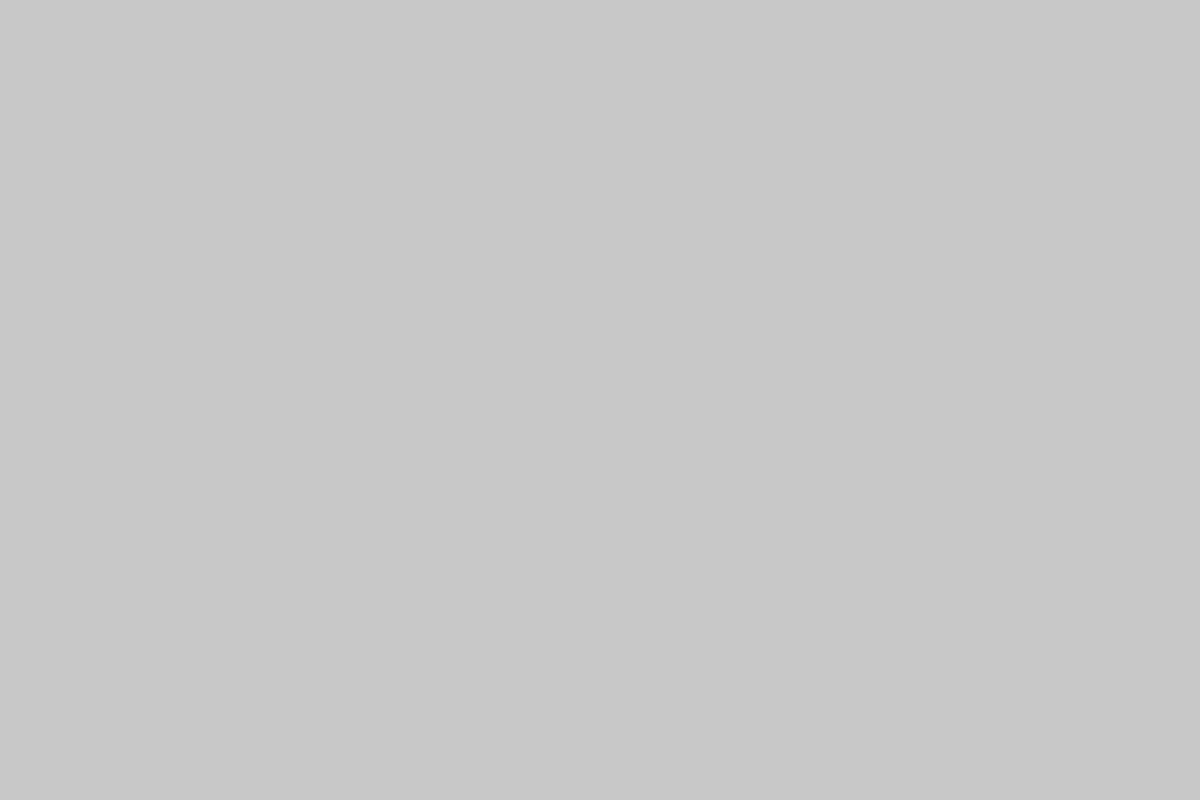
\includegraphics[width=0.63\textwidth,keepaspectratio]{images/ss-09-create-wbp-hud-and-health.png}}
		      \caption{Pembuatan berkas WBP\_HUD dan WBP\_Health di dalam direktori Content/Widget.}
		      \label{fig:ss-create-wbp-hud-and-health}
	      \end{figure}

	\item \textbf{Konfigurasi Progress Bar pada WBP\_Health.} Editor \texttt{WBP\_Health} dibuka. Komponen \textbf{Progress Bar} ditarik dari panel Palette ke dalam hierarki dan dinamai ulang menjadi \textbf{HealthBar}. Melalui panel Details, properti \textbf{Appearance > Fill Color and Opacity} diubah menjadi warna hijau terang, serta properti \textbf{Progress > Percent} disetel ke nilai \textbf{1.0} sebagai kondisi awal darah penuh. Konfigurasi ini ditampilkan pada Gambar \ref{fig:ss-wbp-health-progress-bar}.

	      \begin{figure}[H]
		      \centering
		      \customfbox{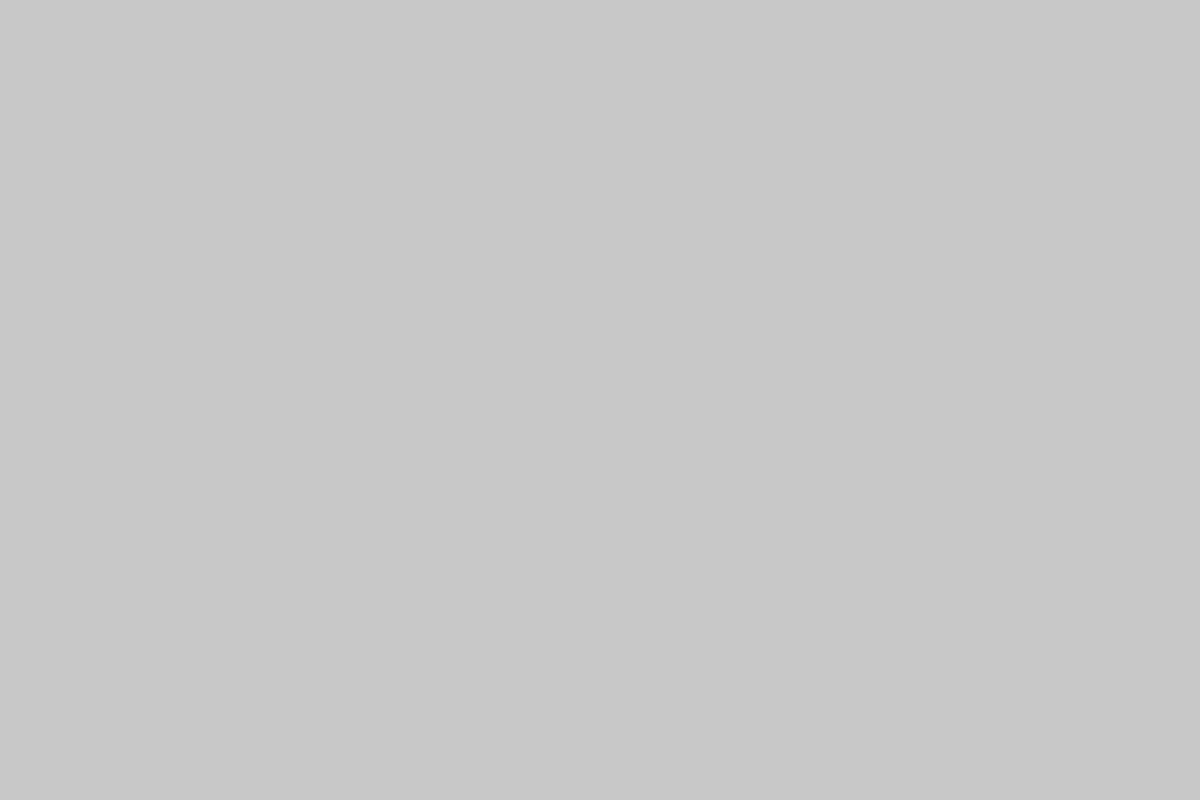
\includegraphics[width=0.63\textwidth,keepaspectratio]{images/ss-10-wbp-health-progress-bar.png}}
		      \caption{Pengaturan warna batang isian dan nilai awal persentase pada komponen HealthBar.}
		      \label{fig:ss-wbp-health-progress-bar}
	      \end{figure}

	\item \textbf{Penyusunan Animasi Getar (onUpdateHealthAnimation).} Pada panel \textbf{Animations}, aset animasi baru bernama \textbf{onUpdateHealthAnimation} ditambahkan. Komponen \texttt{HealthBar} didaftarkan ke linimasa dengan sub-track \textbf{Transform > Translation}. Durasi animasi diatur sepanjang \textbf{0.25 detik} pada kecepatan 20 fps, dengan beberapa keyframe translasi sumbu X dan Y acak untuk menghasilkan efek getaran visual (\textit{shake}) saat darah berkurang, seperti tampak pada Gambar \ref{fig:ss-timeline-onupdatehealthanimation}.

	      \begin{figure}[H]
		      \centering
		      \customfbox{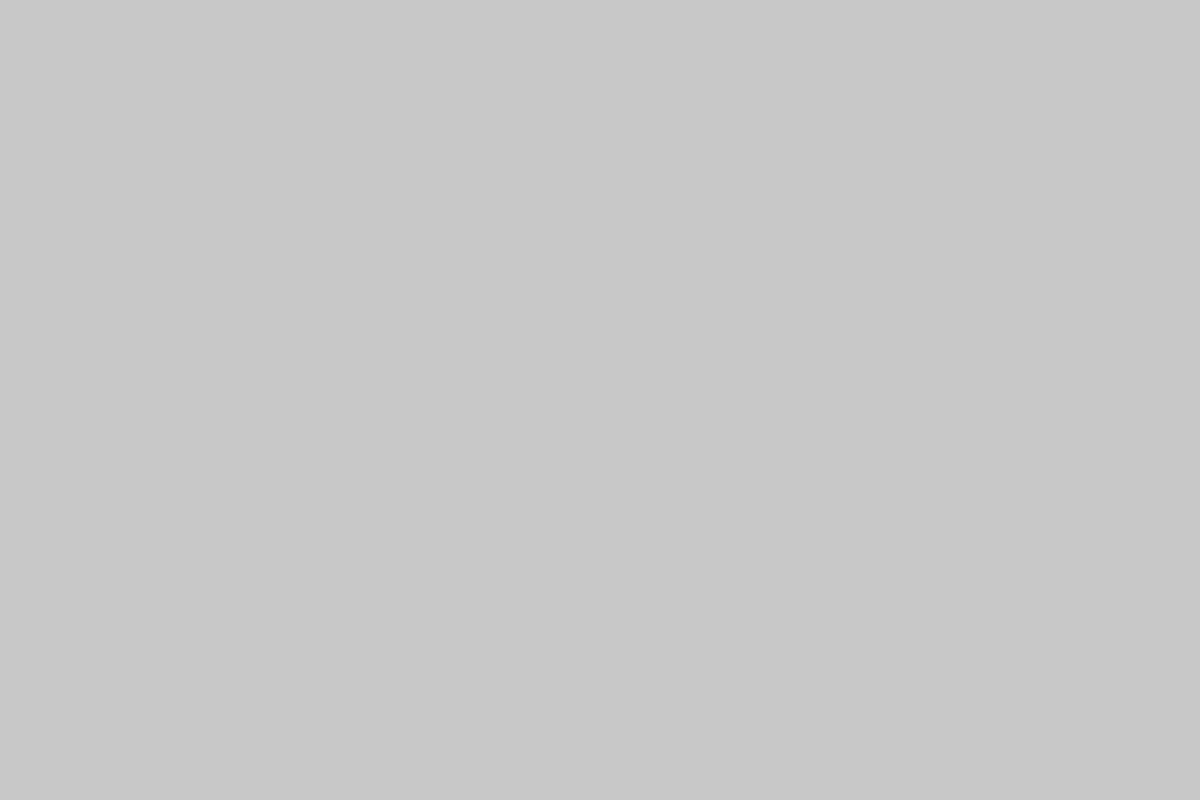
\includegraphics[width=0.63\textwidth,keepaspectratio]{images/ss-11-timeline-onupdatehealthanimation.png}}
		      \caption{Penyusunan linimasa animasi onUpdateHealthAnimation berdurasi 0.25 detik untuk efek getar UI.}
		      \label{fig:ss-timeline-onupdatehealthanimation}
	      \end{figure}

	\item \textbf{Penataan Hierarki Kanvas pada WBP\_HUD.} Editor \texttt{WBP\_HUD} dibuka pada mode Designer. Komponen \textbf{Canvas Panel} ditambahkan sebagai kontainer induk. Selanjutnya, widget \textbf{WBP\_Health} dimasukkan ke dalam Canvas Panel dan diposisikan pada area sudut kiri atas layar dengan margin penjangkaran yang aman dari batas tepi monitor. Penataan hierarki kanvas visual ini diperlihatkan pada Gambar \ref{fig:ss-wbp-hud-canvas-panel-hierarchy}.

	      \begin{figure}[H]
		      \centering
		      \customfbox{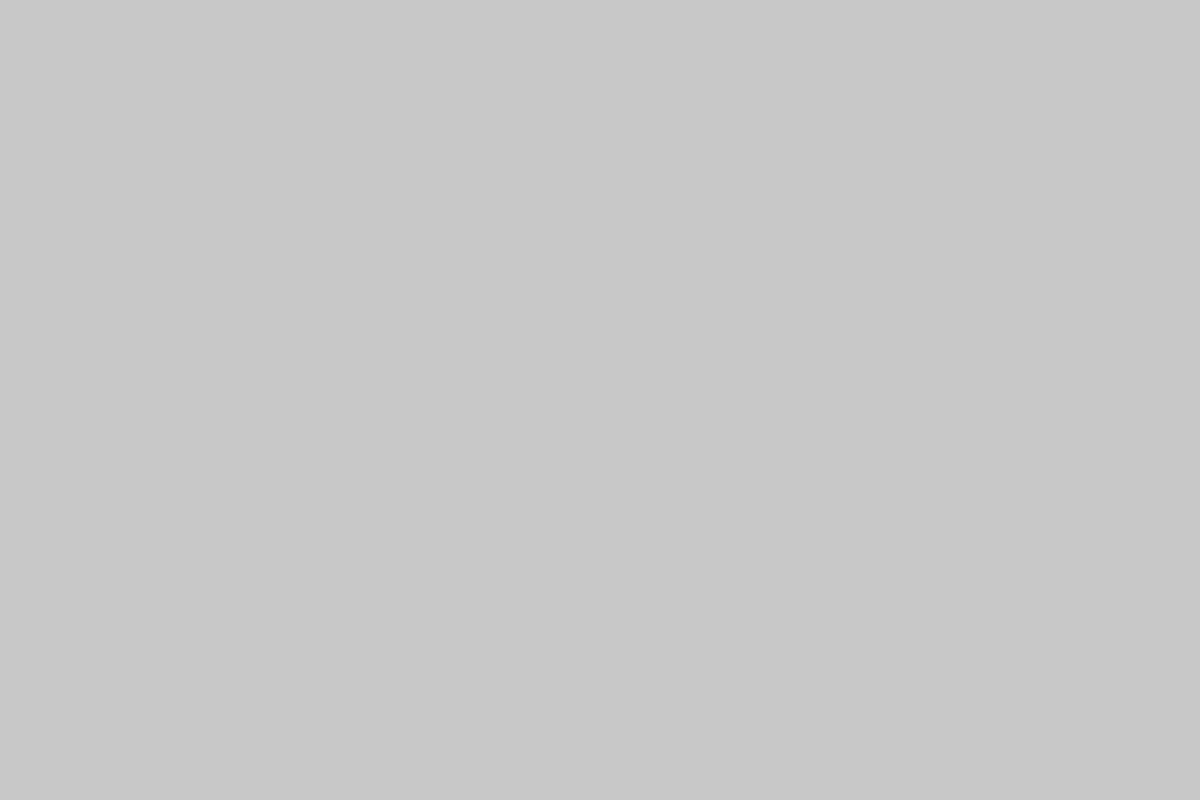
\includegraphics[width=0.63\textwidth,keepaspectratio]{images/ss-12-wbp-hud-canvas-panel-hierarchy.png}}
		      \caption{Penataan letak komponen modular WBP\_Health di dalam Canvas Panel WBP\_HUD pada area kiri atas layar.}
		      \label{fig:ss-wbp-hud-canvas-panel-hierarchy}
	      \end{figure}
\end{enumerate}

\subsection{Pembuatan dan Konfigurasi Blueprint Interface}

\begin{enumerate}\setlength{\itemsep}{0.5em}\setcounter{enumi}{12}
	\item \textbf{Pembuatan Antarmuka BPI\_HUD.} Untuk menyediakan jalur pembaruan nilai darah tanpa ketergantungan langsung ke widget, aset \textit{Blueprint Interface} baru dibuat dengan nama \textbf{BPI\_HUD}. Di dalamnya, fungsi \textbf{UpdateHealthValue} didefinisikan dengan dua parameter input bertipe Float, yaitu \textbf{CurrentHealth} dan \textbf{MaxHealth}, tanpa parameter output. Struktur antarmuka ini tampak pada Gambar \ref{fig:ss-bpi-hud-interface-setup}.

	      \begin{figure}[H]
		      \centering
		      \customfbox{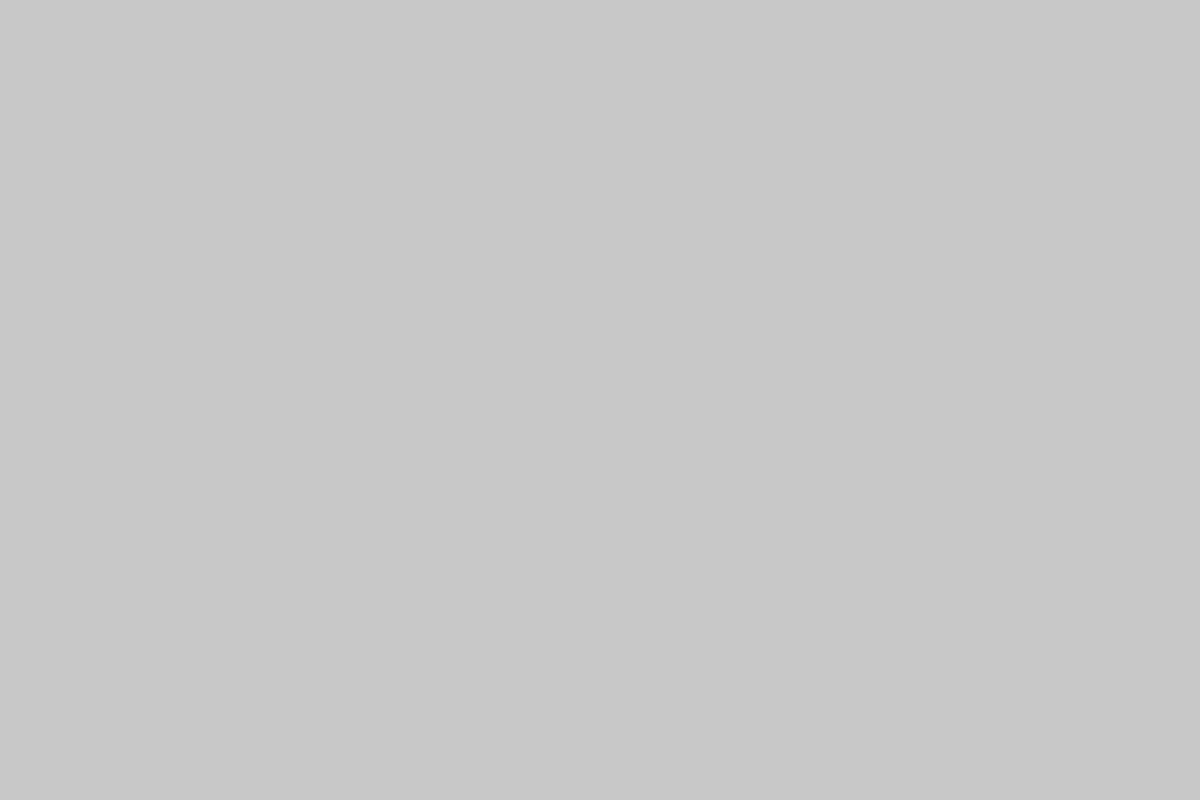
\includegraphics[width=0.63\textwidth,keepaspectratio]{images/ss-13-bpi-hud-interface-setup.png}}
		      \caption{Definisi fungsi UpdateHealthValue pada Blueprint Interface BPI\_HUD dengan parameter input darah.}
		      \label{fig:ss-bpi-hud-interface-setup}
	      \end{figure}

	\item \textbf{Pembuatan Antarmuka BPI\_Widget.} Komunikasi global antara Player Controller, Game Instance, dan karakter dikelola menggunakan antarmuka kedua, yaitu \textbf{BPI\_Widget}. Dua fungsi dideklarasikan: fungsi \textbf{SetHUDWidget} dengan input referensi \texttt{User Widget} (\textbf{HUD}) untuk menyimpan objek widget, serta fungsi \textbf{GetHUDWidget} dengan output referensi \texttt{User Widget} (\textbf{HUD}) untuk mengambil objek widget aktif, seperti diperlihatkan pada Gambar \ref{fig:ss-bpi-widget-interface-setup}.

	      \begin{figure}[H]
		      \centering
		      \customfbox{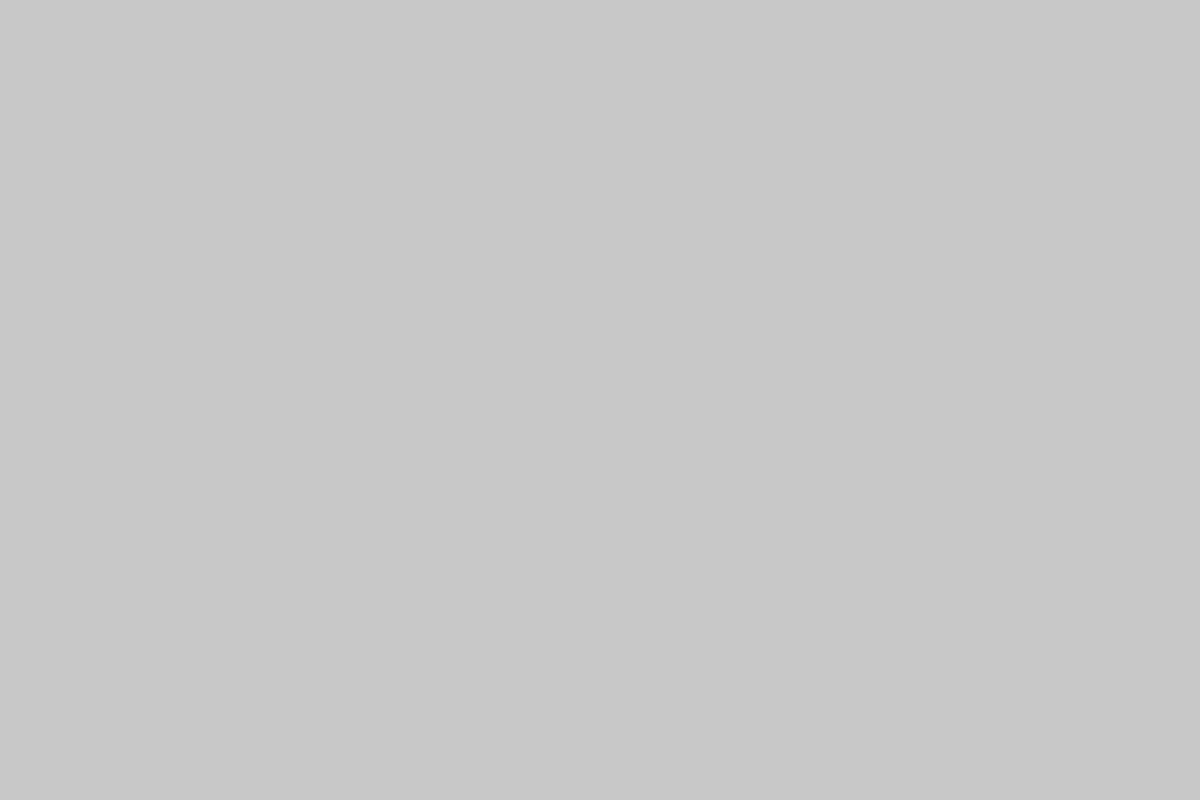
\includegraphics[width=0.63\textwidth,keepaspectratio]{images/ss-14-bpi-widget-interface-setup.png}}
		      \caption{Deklarasi fungsi setter dan getter referensi User Widget pada antarmuka BPI\_Widget.}
		      \label{fig:ss-bpi-widget-interface-setup}
	      \end{figure}
\end{enumerate}

\subsection{Integrasi Logika UI dengan Gameplay dan Komponen Kesehatan}

\begin{enumerate}\setlength{\itemsep}{0.5em}\setcounter{enumi}{14}
	\item \textbf{Implementasi BPI\_HUD pada WBP\_HUD.} Pada editor \texttt{WBP\_HUD}, antarmuka \textbf{BPI\_HUD} didaftarkan melalui \textbf{Class Settings}. Pada Event Graph, fungsi \textbf{Event UpdateHealthValue} diimplementasikan: garis eksekusi memanggil node \textbf{Play Animation} untuk memutar \texttt{onUpdateHealthAnimation} pada instans \texttt{WBP\_Health}, lalu membagi \texttt{CurrentHealth} dengan \texttt{MaxHealth} untuk dihubungkan ke fungsi \textbf{Set Percent} pada komponen \texttt{HealthBar}. Rangkaian logika ini tampak pada Gambar \ref{fig:ss-wbp-hud-event-updatehealthvalue}.

	      \begin{figure}[H]
		      \centering
		      \customfbox{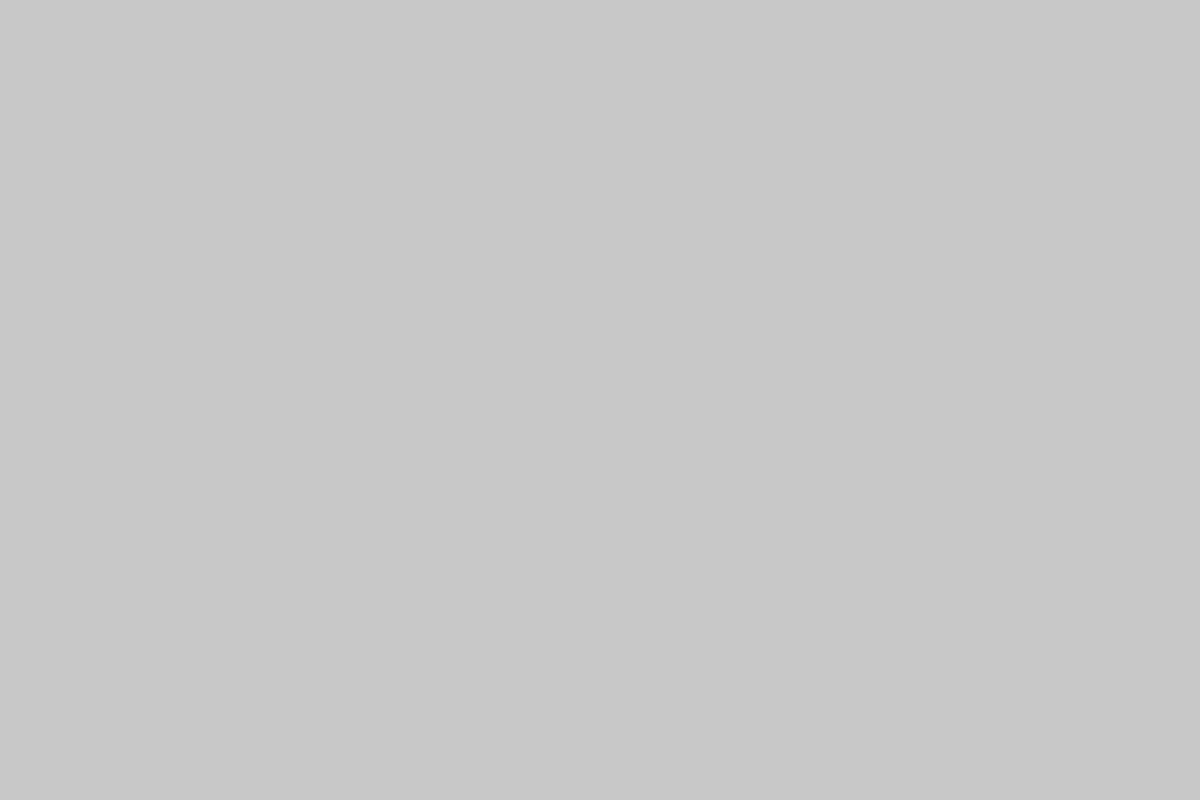
\includegraphics[width=0.63\textwidth,keepaspectratio]{images/ss-15-wbp-hud-event-updatehealthvalue.png}}
		      \caption{Rangkaian Event Graph WBP\_HUD yang memicu pemutaran animasi dan pembaruan persentase HealthBar.}
		      \label{fig:ss-wbp-hud-event-updatehealthvalue}
	      \end{figure}

	\item \textbf{Penyimpanan Referensi Widget di Game Instance.} Blueprint \texttt{BP\_GameInstance} diperbarui dengan menambahkan antarmuka \textbf{BPI\_Widget} pada Class Settings serta mendeklarasikan variabel baru bernama \textbf{AddedWidget} bertipe \textit{User Widget}. Fungsi \textbf{GetHUDWidget} disambungkan langsung untuk mengembalikan nilai variabel tersebut, sementara event \textbf{SetHUDWidget} memperbarui nilai \texttt{AddedWidget} dengan instans widget yang diterima, sebagaimana ditunjukkan pada Gambar \ref{fig:ss-gameinstance-bpi-widget-setup}.

	      \begin{figure}[H]
		      \centering
		      \customfbox{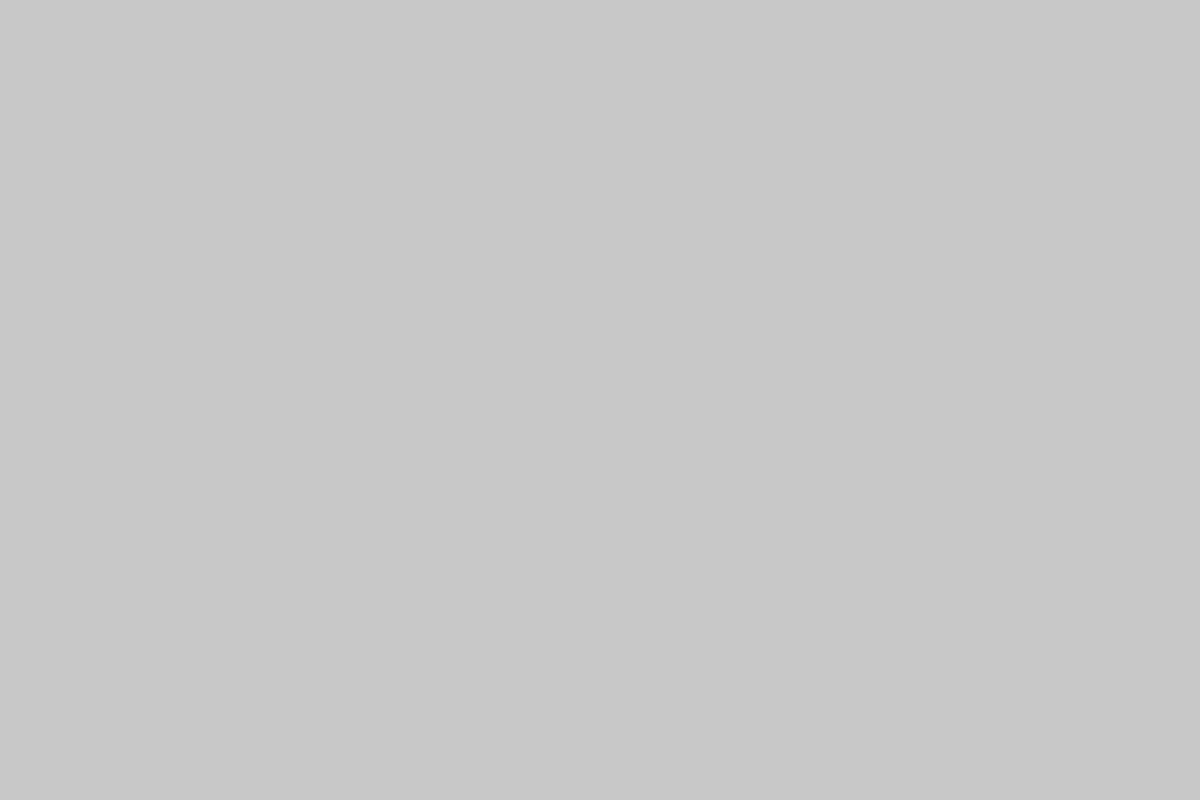
\includegraphics[width=0.63\textwidth,keepaspectratio]{images/ss-16-gameinstance-bpi-widget-setup.png}}
		      \caption{Implementasi fungsi getter dan setter antarmuka BPI\_Widget pada BP\_GameInstance.}
		      \label{fig:ss-gameinstance-bpi-widget-setup}
	      \end{figure}

	\item \textbf{Inisialisasi Pembuatan UI pada Player Controller.} Pada kelas pengontrol karakter \texttt{BP\_ThirdPersonPlayerController}, alur inisialisasi awal disambungkan setelah penetapan konteks input. Node \textbf{Create Widget} dipanggil untuk membuat instans \textbf{WBP\_HUD} dengan \textit{Owning Player} disetel ke \texttt{Self}. Referensi widget yang tercipta dikirim ke Game Instance melalui fungsi pesan \textbf{Set HUDWidget (Target: BPI\_Widget)}, lalu dirender ke layar pemain menggunakan node \textbf{Add to Player Screen}. Rangkaian ini diperlihatkan pada Gambar \ref{fig:ss-playercontroller-create-hud}.

	      \begin{figure}[H]
		      \centering
		      \customfbox{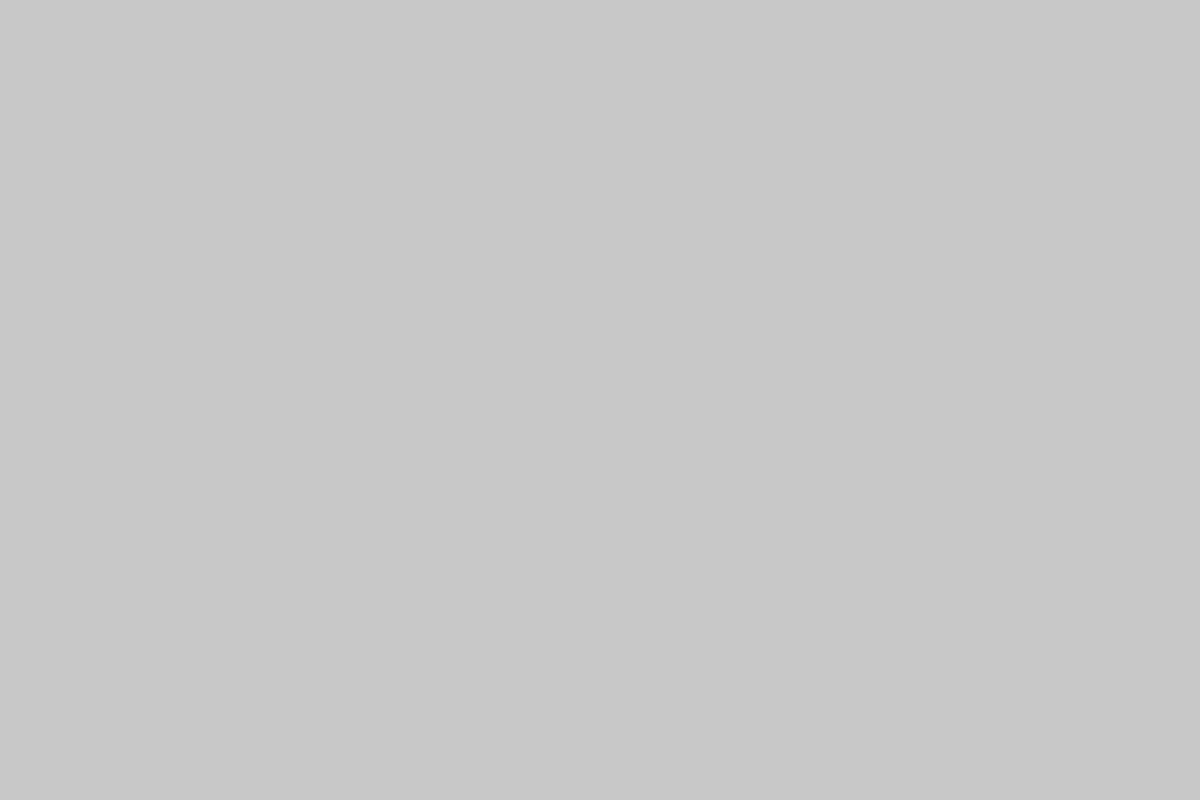
\includegraphics[width=0.63\textwidth,keepaspectratio]{images/ss-17-playercontroller-create-hud.png}}
		      \caption{Alur inisialisasi antarmuka WBP\_HUD dan penampilannya ke layar pemain pada Player Controller.}
		      \label{fig:ss-playercontroller-create-hud}
	      \end{figure}

	\item \textbf{Pembaruan Indikator UI saat Karakter Menerima Kerusakan.} Logika \textbf{Event TakeDamage} pada \texttt{BP\_ThirdPersonCharacter} diperbarui. Setelah komponen kesehatan \texttt{BPC\_Health} mengurangi nilai darah via fungsi \texttt{Modify Health}, alur eksekusi mengambil objek HUD aktif melalui node \textbf{Get Game Instance > Get HUDWidget (Target: BPI\_Widget)}. Pesan interface \textbf{Update Health Value (Target: BPI\_HUD)} kemudian dipanggil dengan memasukkan nilai \texttt{CurrentHealth} dan \texttt{MaxHealth} terbaru dari komponen kesehatan. Alur logika ini ditampilkan pada Gambar \ref{fig:ss-character-takedamage-update-hud}.

	      \begin{figure}[H]
		      \centering
		      \customfbox{
\includegraphics[width=0.63\textwidth,keepaspectratio]{images/ss-18-character-takedamage-update-hud.png}}
		      \caption{Rangkaian Event Graph TakeDamage karakter yang meneruskan data kesehatan terkini ke antarmuka HUD.}
		      \label{fig:ss-character-takedamage-update-hud}
	      \end{figure}
\end{enumerate}

\clearpage

\section{Hasil Akhir}
Pengujian sistem terintegrasi dilakukan langsung di dalam editor Unreal Engine 5.8 dengan membuka level \textbf{LV\_Praktikum} dan menekan tombol \textbf{Play} (PIE). Saat sesi permainan dimulai, antarmuka HUD (\texttt{WBP\_HUD}) berhasil dimunculkan secara otomatis di sudut kiri atas layar pemain dengan indikator bilah darah (\texttt{HealthBar}) berwarna hijau terang dalam kondisi terisi penuh (100\%).

\begin{figure}[H]
	\centering
	\customfbox{
\includegraphics[width=0.82\textwidth,keepaspectratio]{images/ss-19-hasil-akhir-gameplay-ui-healthbar.png}}
	\caption{Uji coba gameplay di level LV\_Praktikum: indikator HealthBar hijau muncul di kiri atas, berkurang dan memainkan animasi getar saat karakter menerima damage tabrakan.}
	\label{fig:hasil-akhir-gameplay}
\end{figure}

Ketika karakter digerakkan menabrak aktor pemicu bahaya (\textit{hazard collision}), logika penanganan tabrakan memicu fungsi \texttt{Modify Health} pada \texttt{BPC\_Health}. Secara instan, alur interface mengirimkan data darah terbaru menuju sistem HUD melalui Game Instance. Panjang visual batang \texttt{HealthBar} langsung menyusut proporsional terhadap sisa darah, dibarengi dengan pemutaran animasi getaran (\textit{shake translation}) berdurasi 0,25 detik pada bilah antarmuka. Karakter tetap dapat bergerak secara responsif di atas bentang alam berkontur yang dihiasi oleh pepohonan foliage tanpa mengalami penurunan performa grafis, membuktikan seluruh integrasi modul praktikum telah berfungsi sempurna sesuai spesifikasi.

\clearpage

\chapter{Kesimpulan}
Praktikum Pertemuan 7 memberikan pemahaman komprehensif mengenai alur integrasi aset digital eksternal dari marketplace Fab, penataan material bentang alam multi-layer, sebaran vegetasi lingkungan melalui sistem foliage, serta arsitektur antarmuka pemain modular menggunakan UMG dan Blueprint Interface pada Unreal Engine 5.8. Pemanfaatan paket aset dari platform Fab terbukti mempercepat pembentukan lingkungan visual berkualitas tinggi, di mana mekanisme pemilihan versi kompatibel memungkinkan integrasi paket versi terdahulu ke dalam engine mutakhir tanpa kendala struktural.

Penerapan instans material \texttt{MI\_landscape\_pro\_v2\_inst} yang didukung kontainer data \textit{Layer Info} berhasil memfasilitasi pengecatan multi-tekstur tanah, rumput, dan genangan air secara fleksibel dengan perhitungan blending bobot yang akurat. Kombinasi metode penempatan vegetasi manual untuk pohon-pohon signifikan dan pemanfaatan \textit{Foliage Mode} untuk sebaran vegetasi massal berbasis instansiasi HISM menghadirkan lingkungan alam yang rimbun namun tetap optimal dalam penggunaan beban pemanggilan penggambaran grafis.

Pembangunan antarmuka pemain berbasis UMG yang dipisahkan secara modular ke dalam \texttt{WBP\_HUD} dan \texttt{WBP\_Health} berhasil mewujudkan tata kelola hierarki visual yang rapi. Pemanfaatan pola desain \textit{Blueprint Interface} (\texttt{BPI\_HUD} dan \texttt{BPI\_Widget}) yang dipadukan dengan persistensi \textit{Game Instance} mengeliminasi kebutuhan pemanggilan \textit{hard-casting} yang kaku. Ketika karakter menerima kerusakan, data kesehatan diteruskan secara terisolasi untuk memperbarui persentase \texttt{HealthBar} dan memicu animasi getar responsif secara seketika, mengonfirmasi seluruh tujuan pembelajaran praktikum telah tercapai dengan sangat baik.

\clearpage

\addcontentsline{toc}{chapter}{Daftar Pustaka}
\renewcommand{\bibname}{Daftar Pustaka}
\begin{spacing}{0.95}
	\begin{thebibliography}{99}
		\setlength{\itemsep}{0.08em}
		\bibitem{modul7} Tim Dosen Praktikum Pengembangan Game, ``Modul Praktikum Pengembangan Game Pertemuan 7: Asset FAB dan Widget Blueprint (UI)'', Departemen Teknik Elektro dan Informatika, Sekolah Vokasi, Universitas Gadjah Mada, Yogyakarta, 2026.
		\bibitem{fab-market} Epic Games, ``About Fab: The Unified Digital Marketplace for Creators'', 2026. [Daring]. Tersedia: \url{https://web.archive.org/web/20241022142230/https://www.fab.com/o/about}.
		\bibitem{epic-fab-overview} Epic Games, ``Unreal Engine Fab Marketplace Overview'', Epic Developer Community, 2026. [Daring]. Tersedia: \url{https://dev.epicgames.com/community/learning/talks-and-demos/mJy4/unreal-engine-fab-marketplace-overview}.
		\bibitem{epic-landscape-materials} Epic Games, ``Landscape Materials in Unreal Engine'', Unreal Engine 5.8 Documentation, 2026. [Daring]. Tersedia: \url{https://dev.epicgames.com/documentation/en-us/unreal-engine/landscape-materials-in-unreal-engine}.
		\bibitem{epic-foliage-mode} Epic Games, ``Foliage Mode in Unreal Engine'', Unreal Engine 5.8 Documentation, 2026. [Daring]. Tersedia: \url{https://dev.epicgames.com/documentation/en-us/unreal-engine/foliage-mode-in-unreal-engine}.
		\bibitem{epic-umg} Epic Games, ``UMG UI Designer in Unreal Engine'', Unreal Engine 5.8 Documentation, 2026. [Daring]. Tersedia: \url{https://dev.epicgames.com/documentation/en-us/unreal-engine/umg-ui-designer-in-unreal-engine}.
		\bibitem{epic-widget-animation} Epic Games, ``Animating UMG Widgets in Unreal Engine'', Unreal Engine 5.8 Documentation, 2026. [Daring]. Tersedia: \url{https://dev.epicgames.com/documentation/en-us/unreal-engine/animating-umg-widgets-in-unreal-engine}.
		\bibitem{epic-blueprint-interface} Epic Games, ``Blueprint Interfaces in Unreal Engine'', Unreal Engine 5.8 Documentation, 2026. [Daring]. Tersedia: \url{https://dev.epicgames.com/documentation/en-us/unreal-engine/blueprint-interface-in-unreal-engine}.
		\bibitem{epic-game-instance} Epic Games, ``Game Instance Subsystems in Unreal Engine'', Unreal Engine 5.8 Documentation, 2026. [Daring]. Tersedia: \url{https://dev.epicgames.com/documentation/en-us/unreal-engine/game-instance-subsystems-in-unreal-engine}.
	\end{thebibliography}
\end{spacing}

\end{document}
